\documentclass[10pt,a4paper]{article}
\usepackage[margin=.7cm]{geometry}
\usepackage[utf8]{inputenc}
\usepackage[IL2]{fontenc}
\usepackage[czech]{babel}
\usepackage{microtype}
\usepackage{amssymb}
\usepackage{amsthm}
\usepackage{amsmath}
\usepackage{xcolor}
\usepackage{graphicx}
\usepackage{tikz}
\usetikzlibrary{shapes,arrows}

\usepackage[inline]{enumitem}

\setlist[enumerate]{label={(\alph*)},topsep=\smallskipamount,itemsep=\smallskipamount,parsep=0pt}
\setlist[itemize]{topsep=\smallskipamount,noitemsep}

\def\tisk{%
\newbox\shipouthackbox
\pdfpagewidth=2\pdfpagewidth
\let\oldshipout=\shipout
\def\shipout{\afterassignment\zdvojtmp \setbox\shipouthackbox=}%
\def\zdvojtmp{\aftergroup\zdvoj}%
\def\zdvoj{%
    \oldshipout\vbox{\hbox{%
        \copy\shipouthackbox
        \hskip\dimexpr .5\pdfpagewidth-\wd\shipouthackbox\relax
        \box\shipouthackbox
    }}%
}}%


\newtheorem*{poz}{Pozorování}

\theoremstyle{definition}
\newtheorem{uloha}{Úloha}
\newtheorem{suloha}[uloha]{\llap{$\star$ }Úloha}
\newtheorem*{bonus}{Bonus}
\newtheorem*{defn}{Definice}

\pagestyle{empty}

\let\ee\expandafter

\def\vysld{}
\let\printvysl\relax
\let\printalphvysl\relax

\makeatletter
\def\vyslplain#1{\ee\ee\ee\gdef\ee\ee\ee\vysld\ee\ee\ee{\ee\vysld\ee\printvysl\ee{\the\c@uloha}{#1}}}
\let\vysl\vyslplain

\def\locvysl#1{\ee\gdef\ee\locvysld\ee{\locvysld\item #1}}
\let\lv\locvysl

\newenvironment{ulohav}[1][]{\begin{uloha}[#1]\gdef\locvysld{\begin{enumerate}}}{\ee\vyslplain\ee{\locvysld\end{enumerate}}\end{uloha}}
\newenvironment{sulohav}[1][]{\begin{suloha}[#1]\gdef\locvysld{\begin{enumerate*}}}{\ee\vyslplain\ee{\locvysld\end{enumerate*}}\end{suloha}}

\makeatother

\tikzstyle{prohr}=[diamond]
\tikzstyle{vyhr}=[star,star points=8]

\tikzset{every node/.style={draw,circle,inner sep=1pt,minimum width={width("M")+4pt},minimum height={height("M")+2pt}}, >=latex'}

\newcommand{\stav}[3][]{\node[#1] (#2) at (#3) {#2};}
\def\tbr{to [bend right]}
\def\tbl{to [bend left]}
\def\cn#1#2{\draw[->] (#1) to (#2);}
\def\cnr#1#2{\draw[->] (#1) \tbr (#2);}
\def\cnl#1#2{\draw[->] (#1) \tbl (#2);}
\newcommand{\ctkz}[2][]{$\vcenter{\hbox{\begin{tikzpicture}[#1]#2\end{tikzpicture}}}$}

\newcommand{\nstav}[4][]{\node[#1] (#2) at (#3) {$#4{}$};}


\newcount\colorct
\def\addcolor#1{\advance\colorct1\relax\expandafter\definecolor\expandafter{\the\colorct clr}{rgb}{#1}}
\addcolor{0,0,0}
\addcolor{0.,0.,0.}\addcolor{0.996078,0.360784,0.027451}\addcolor{0.996078,0.988235,0.0352941}\addcolor{0.541176,0.713725,0.027451}\addcolor{0.145098,0.435294,0.384314}\addcolor{0.00784314,0.509804,0.929412}\addcolor{0.152941,0.113725,0.490196}\addcolor{0.470588,0.262745,0.584314}\addcolor{0.890196,0.0117647,0.490196}\addcolor{0.905882,0.027451,0.129412}\addcolor{0.,0.,0.}\addcolor{0.996078,0.360784,0.027451}\addcolor{0.996078,0.988235,0.0352941}\addcolor{0.541176,0.713725,0.027451}\addcolor{0.145098,0.435294,0.384314}\addcolor{0.00784314,0.509804,0.929412}\addcolor{0.152941,0.113725,0.490196}\addcolor{0.470588,0.262745,0.584314}\addcolor{0.890196,0.0117647,0.490196}\addcolor{0.905882,0.027451,0.129412}\addcolor{0.,0.,0.}\addcolor{0.996078,0.360784,0.027451}\addcolor{0.996078,0.988235,0.0352941}\addcolor{0.541176,0.713725,0.027451}\addcolor{0.145098,0.435294,0.384314}\addcolor{0.00784314,0.509804,0.929412}\addcolor{0.152941,0.113725,0.490196}\addcolor{0.470588,0.262745,0.584314}\addcolor{0.890196,0.0117647,0.490196}\addcolor{0.905882,0.027451,0.129412}\addcolor{0.,0.,0.}\addcolor{0.996078,0.360784,0.027451}\addcolor{0.996078,0.988235,0.0352941}\addcolor{0.541176,0.713725,0.027451}\addcolor{0.145098,0.435294,0.384314}\addcolor{0.00784314,0.509804,0.929412}\addcolor{0.152941,0.113725,0.490196}\addcolor{0.470588,0.262745,0.584314}\addcolor{0.890196,0.0117647,0.490196}\addcolor{0.905882,0.027451,0.129412}

\begin{document}

%\tisk

\section*{Teorie her}


\begin{ulohav}
Určete, které pozice jsou v následujících hrách vyhrávající (tzn. hráč na tahu při ideální hře určitě vyhraje) a které prohrávající. Hvězda značí koncovou vyhrávající pozici, čtverec prohrávající, ostatní je potřeba dopočítat.
%\vskip-2\bigskipamount\vskip0pt
\begin{flushleft}
\begin{enumerate*}[itemjoin=\quad]
\item \ctkz[scale=1.2]{%
\stav[vyhr]{A}{0,0}
\stav[prohr]{B}{0,1}
\stav{C}{1,0}
\stav{D}{1,1}
\stav{E}{2,0}
\stav{F}{2,1}
\stav{G}{3,0}
\stav{H}{3,1}
\stav{I}{4,0}
\stav{J}{4,1}
\stav{K}{5,0}
\stav{L}{5,1}
\cn CA
\cn DB
\cn FD
\cn FC
\cn EC
\cn HF
\cn GE
\cn GF
\cnr JF
\cnl IE
\cn KI
\cn LJ
\cn KJ
\cn JH
\cn IG
\cn JG
\cn IH}\lv{vyhrávající: A, D, E, F, I, J}
%
%
\item \ctkz[scale=1.2]{%
\stav[prohr]{A}{0,1}
\stav{B}{1,0} \cn BA
\stav{C}{1,1} \cn CA
\stav{D}{1,2} \cn DA
\cn DC \cn BC
\stav{E}{2,1} \cn ED \cn EB
\stav{F}{2.8,0} \cn FB \cn FC
\stav{G}{2.8,2} \cn GD \cn GC
\stav{H}{3,1} \cn HE
\stav{I}{4,0} \cn IH \cnl IB
\stav{J}{4,2} \cn JH \cnr JD
\stav{K}{5,.6} \cn KG \cn KF
\stav{L}{5,1.4} \cn LF \cn LG
\stav{M}{6,0} \cn MK \cnl MF
\stav{N}{6,2} \cn NL \cnr NG
\stav{O}{6,1} \cnr OJ \cnl OI
\stav{P}{7,1} \cn PM \cn PN \cn PO
}\lv{vyhrávající: B, C, D, H, K, L, M, N, O}
%
%
\item \ctkz[yscale=1.5,xscale=4]{%
\stav{A}{0,0}
\stav[vyhr]{B}{1,0}
\stav{C}{2,0}
\stav{D}{3,0}
\stav{E}{0,1}
\stav{F}{1,1}
\stav{G}{2,1}
\stav{H}{3,1}
\stav{I}{0,2}
\stav{J}{1,2}
\stav{K}{2,2}
\stav{L}{3,2}
\stav{M}{0,3}
\stav{N}{1,3}
\stav{O}{2,3}
\stav[prohr]{P}{3,3}
\colorct=0
\def\cnr#1#2{\advance\colorct1\relax\draw[->,draw=\the\colorct clr] (#1) \tbr (#2);}
\def\cnl#1#2{\advance\colorct1\relax\draw[->,draw=\the\colorct clr] (#1) \tbl (#2);}
\cnl AP \cnr CA \cnr CG \cnr CK \cnr CL \cnr CP \cnl DE \cnr DP \cnr EA \cnr EG \cnr EO \cnr EP \cnr FA \cnr FD \cnr FE \cnr FL \cnr GO \cnr GP \cnl HC \cnl HF \cnr IJ \cnr JL \cnr KB \cnl KD \cnr KG \cnr LA \cnr LB \cnl LG \cnr LO \cnr LP \cnr MA \cnr MD \cnr MH \cnr MJ \cnl MP \cnr NA \cnr NE \cnr NH \cnr OP
}\lv{vyhrávající: A, B, C, D, E, G, H, I, L, M, O}
\end{enumerate*}
\end{flushleft}
\end{ulohav}

\begin{ulohav}
V pravém horním rohu šachovnice $8 \times 8$ stojí
\begin{enumerate}
    \item jednostranná věž (může se pohybovat jen doleva nebo dolů o libovolný počet polí),\lv{prohrávající jsou přesně pole na diagonále}
    \item jednostranný král (může se pohybovat právě o jedno pole dolů, doleva nebo doleva dolů).\lv{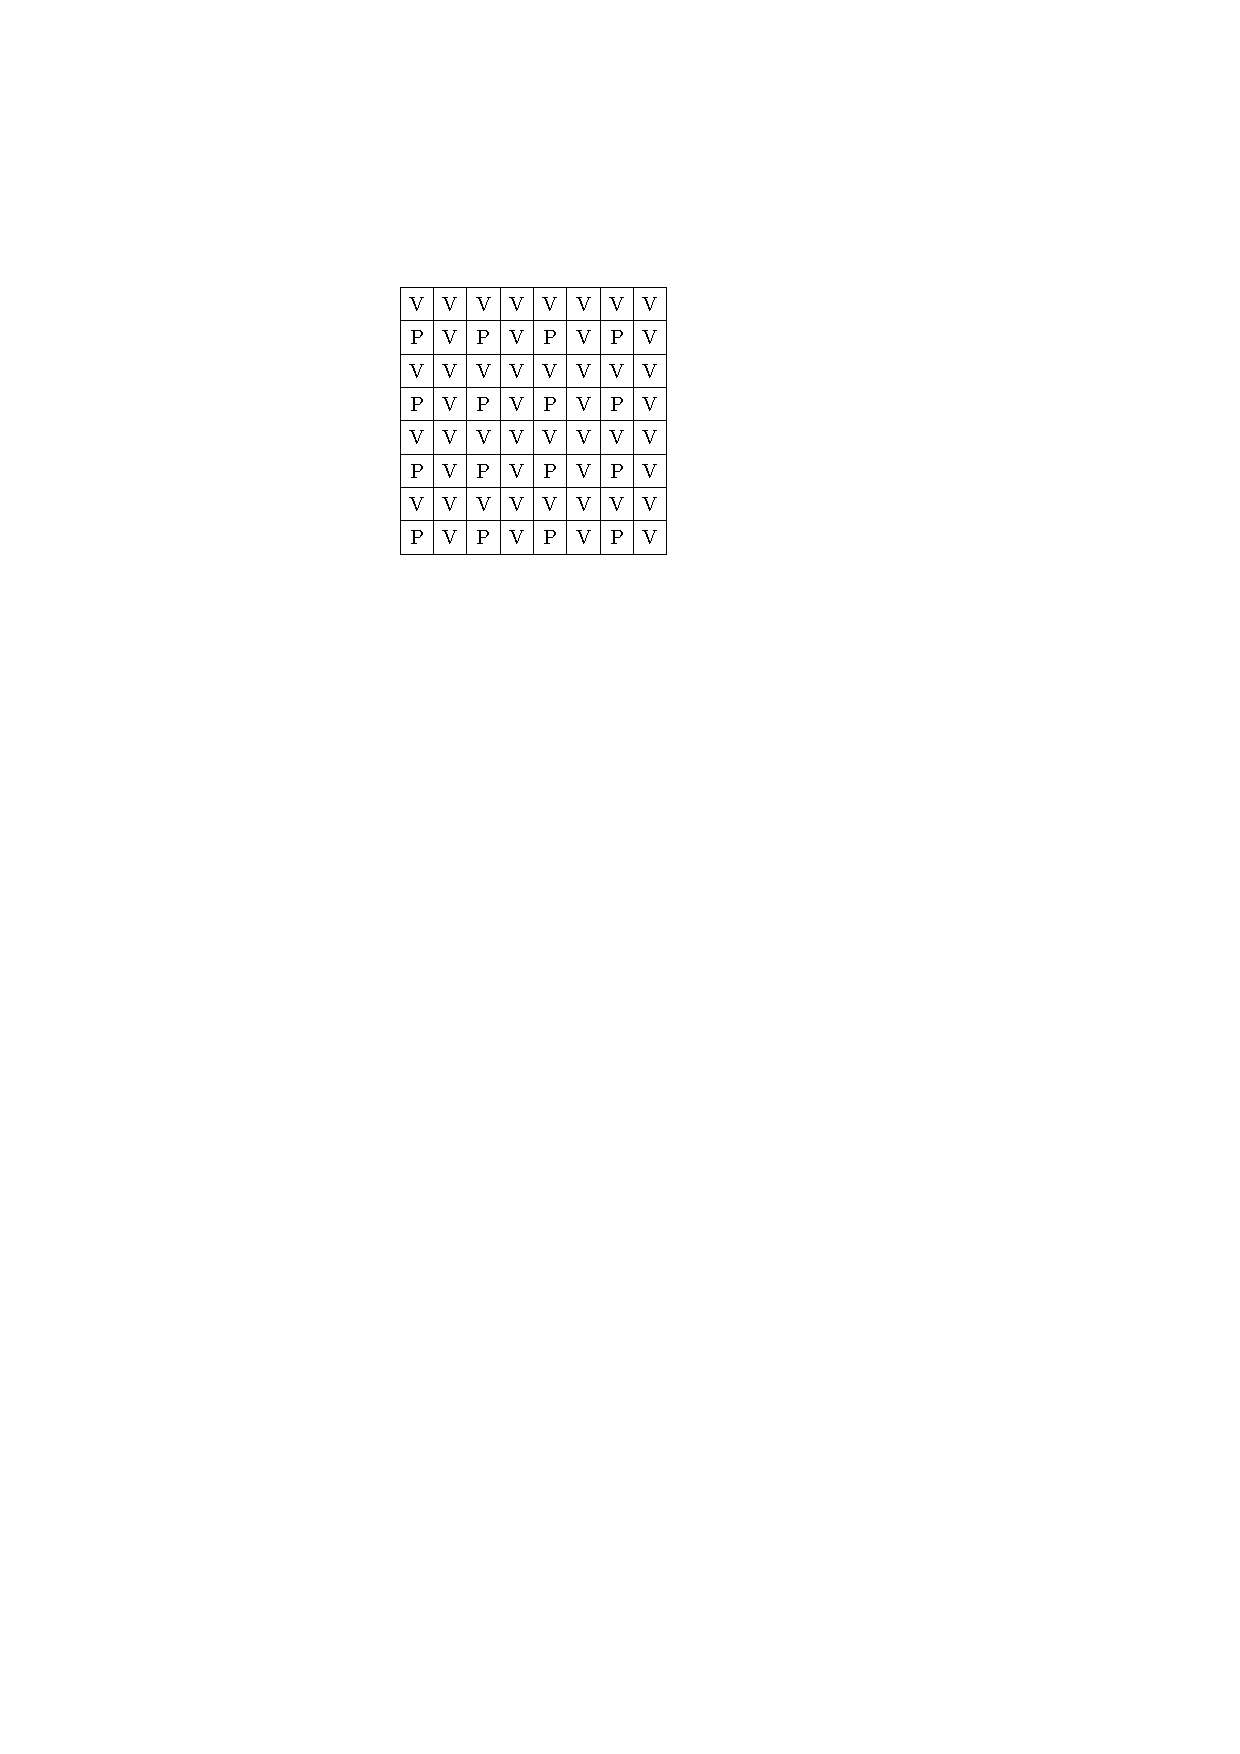
\includegraphics{kral_rozbor.pdf} (prohrávající = obě souřadnice liché, pokud je levý dolní roh $(1,1)$)}
\end{enumerate}
Hráči se střídají v tazích, kdo nemůže táhnout, prohrál. Určete, které pozice jsou vyhrávající a které prohrávající.
\end{ulohav}


\begin{ulohav}
Na stole jsou dvě hromádky ($A$ a $B$) o pěti sirkách. V jednom tahu můžeme brát sirky pouze z jedné hromádky. Kdo nemůže táhnout, prohrál. Určete, které pozice jsou vyhrávající a prohrávající, pokud
\begin{enumerate}
    \item v jednom tahu můžeme z $A$ nebo $B$ odebrat jednu nebo dvě sirky,\lv{prohrávající jsou ty se stejným počtem sirek na obou hromádkách}
    \item v jednom tahu můžeme z $A$ nebo $B$ odebrat jednu až tři sirky,\lv{prohrávající jsou ty se stejným počtem sirek na obou hromádkách}
    \item v jednom tahu můžeme z $A$ odebrat jednu nebo dvě sirky, nebo z $B$ jednu až tři sirky.\lv{prohrávající jsou tyto $(A, B)$: $(0,0)$, $(3,0)$, $(1,1)$, $(4,1)$, $(2,2)$, $(5,2)$, $(4, 0)$, $(3,4)$, $(1,5)$, $(4,5)$}
\end{enumerate}
\end{ulohav}


\begin{uloha}
Vedle sebe je napsaných $n$ mínůsu. V jednom tahu hráč přepíše buď jeden, nebo dva sousední mínusy na plusy. Hráči se střídají, kdo nemůže táhnout, prohrál. Kdo vyhraje? (Zkuste si pro malé hodnoty $n$, potenciálně zkuste přijít na obecný výsledek pro všechna $n$.)\vysl{pro $n > 0$ vždy začínající hráč vyhraje; hraje tak, že nejprve tahem doprostřed to rozdělí na dvě \uv{sekce} o stejné velikosti a následně opakuje to, co dělá druhý hráč, aby po jeho tahu byly obě sekce stejné}
\end{uloha}


\hbox to\hsize{\vbox{%
\linewidth=.5\linewidth
\hsize=.5\hsize
\begin{ulohav}
V této hře (diagram vpravo) proti sobě hrají Max a Mína. Začínají na políčku se srdíčkem a střídavě se pohybují po šipkách, dokud nedojedou do místa s číslem. Maxův cíl je skončit na políčku s co nejvyšším číslem, naopak Mína chce co nejmenší. Rozhodněte, jaký bude finální výsledek, pokud je první na tahu \begin{enumerate*}
    \item Max,\lv{6}
    \item Mína.\lv{2}
\end{enumerate*}
\end{ulohav}}\hfil
\hbox{%
\begin{tikzpicture}
    \nstav{S}{0,.5}{\heartsuit}
    \nstav{A}{1,0}{} \cn SA
    \nstav{B}{1,1}{} \cn SB

    \nstav{E}{2,-1}{} \cn AE
    \nstav{F}{2.5,0.2}{} \cn AF
    \nstav{G}{2.5,.8}{} \cn BG
    \nstav{H}{2,2}{} \cn BH

    \nstav{aa}{3,-1}{4} \cn E{aa}
    \nstav{bb}{3,-.5}{9} \cn E{bb}
    \nstav{cc}{4,-.5}{5} \cn F{cc}
    \nstav{dd}{4,0}{6} \cn F{dd}
    \nstav{ee}{4,1}{2} \cn G{ee}
    \nstav{ff}{4,1.5}{3} \cn G{ff}
    \nstav{gg}{3,1.5}{2} \cn H{gg}
    \nstav{hh}{3,2}{6} \cn H{hh}


    \nstav{C}{-1,0}{} \cn SC
    \nstav{D}{-1,1}{} \cn SD

    \nstav{I}{-2,-1}{} \cn CI
    \nstav{J}{-2.5,.2}{} \cn CJ
    \nstav{K}{-2.5,.8}{} \cn DK
    \nstav{L}{-2,2}{} \cn DL

    \nstav{ii}{-3,-1}{1} \cn I{ii}
    \nstav{jj}{-3,-.5}{0} \cn I{jj}
    \nstav{kk}{-4,-.5}{2} \cn J{kk}
    \nstav{ll}{-4,0}{5} \cn J{ll}
    \nstav{mm}{-4,1}{2} \cn K{mm}
    \nstav{nn}{-4,1.5}{3} \cn K{nn}
    \nstav{oo}{-3,1.5}{7} \cn L{oo}
    \nstav{pp}{-3,2}{5} \cn L{pp}

\end{tikzpicture}
}}



\hbox to\hsize{\vbox{%
\linewidth=.72\linewidth
\hsize=.72\hsize
\begin{ulohav}
Opět proti sobě hrají Max a Mína. Začínají s figurkou v levém dolním rohu šachovnice, střídají se v tazích figurkou, hra končí, jakmile někdo z~nich táhne na políčko s~číslem. Maxův cíl je skončit na políčku s co nejvyšším číslem, naopak Mína chce co nejmenší.
Rozhodněte, jaký bude finální výsledek, pokud jejich figurkou je
\begin{enumerate}
    \item princ (může táhnout jenom o jedna nahoru, nebo o jedna doprava),\lv{začíná Max: 7, začíná Mína: 4}
    \item jednostranná věž (může táhnout o libovolný počet polí nahoru, nebo o libovolný počet doprava),\lv{začíná Max: 9, začíná Mína: 2}
    \item jednostranný král (může táhnout jenom o jedna nahoru, o jedna doprava nebo o jedna doprava nahoru).\lv{začíná Max: 7, začíná Mína: 4}
\end{enumerate}
Pro každou figuru rozeberte situaci, kdy začíná Max i kdy začíná Mína.
\end{ulohav}}\hfil
\hbox{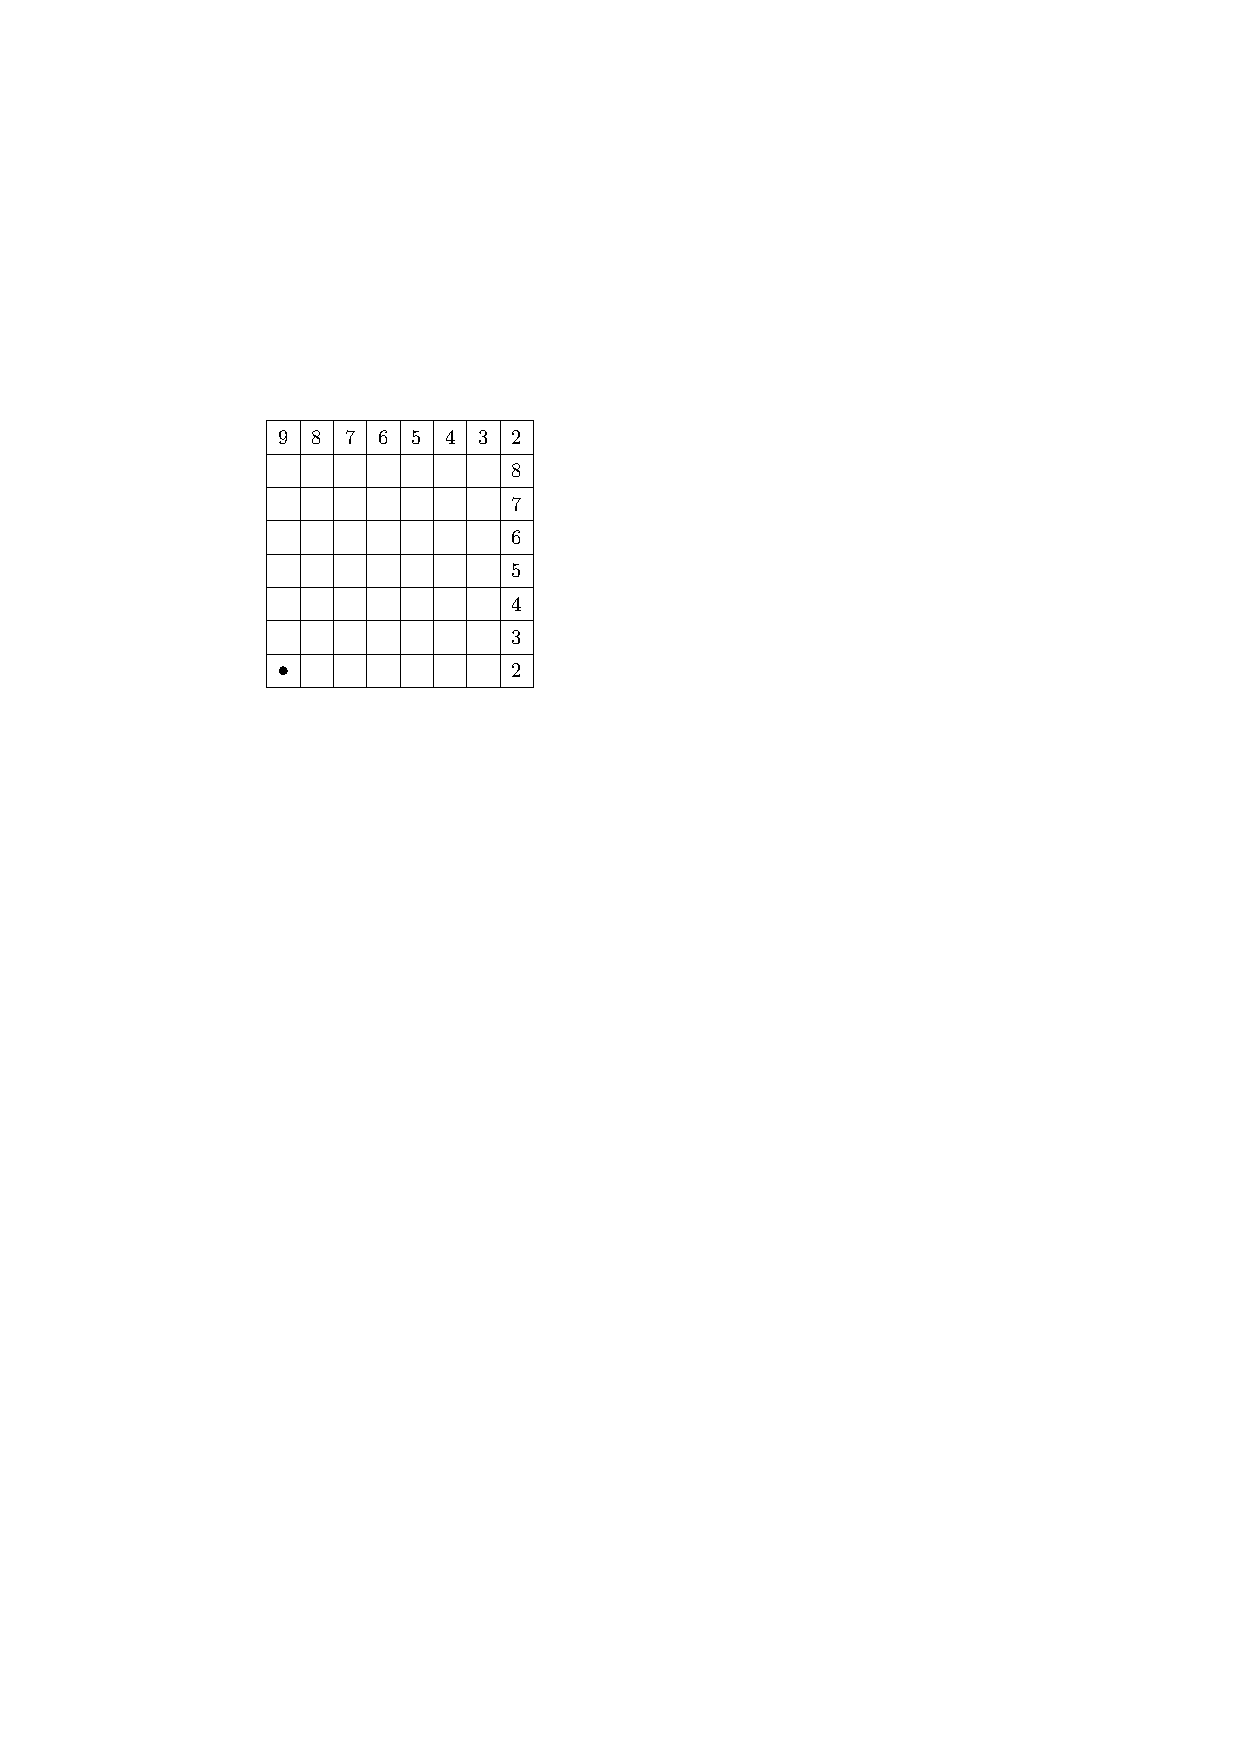
\includegraphics{sachovnice_minimax.pdf}}%
}


\begin{suloha}
Rozmyslete si, že \emph{minimaxový algoritmus} z předchozích dvou úloh je vlastně stejně aplikovatelný i na úlohy o vyhrávajících a prohrávajících pozicích, pokud přidělíme vhodné \uv{ceny} pozic.
\end{suloha}


\newpage
\parindent=0pt
\parskip=\smallskipamount
\def\printvysl#1#2{\textbf{#1.}\ #2\par}
\def\printalphvysl#1#2#3{\textbf{#1}(#2)\ #3\par}
\vysld



\end{document}